
\section{Data Preparation}
\label{sec:data_prep}
Kaggle is a public platform which provides various types of data for research purpose. The dataset `foodRecSys-V1' used in this thesis is received from Kaggle \cite{48}. This dataset contains recipes and ratings crawled from `Allrecipes.com'. It consists of three files. The `core-data\_recipe.csv' file has all information about recipes such as `recipe\_id', `recipe\_name', `image\_url', `ingredients', `cooking\_directions', `nutritions' as shown in \autoref{fig:raw_recipes_head}. It has $45630$ recipes with $6$ columns.
\begin{singlespace}
\begin{figure}[H]
	\centering
	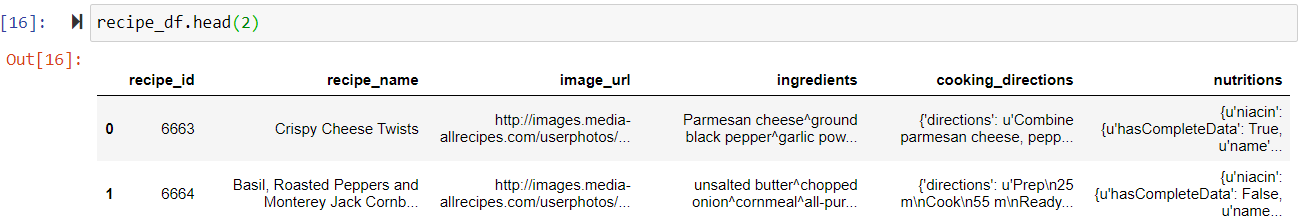
\includegraphics[width=1.0\linewidth]{raw_recipes_head}
	\caption{Raw Recipe Data}
	\label{fig:raw_recipes_head}
\end{figure}
\end{singlespace}

\noindent The other two files `core-data-train\_rating.csv' and `core-data-test\_rating.csv' provide user interactions with recipes. User interaction refers to a record in the file where a user has given a rating to at least one recipe. As shown in \autoref{fig:raw_ratings_head}, user - 5215572 has given ratings to two recipes. These two files are combined into a single file that has all user interactions.  Total user recipe interactions in this merged file are $960386$. 

\begin{singlespace}
\begin{figure}[H]
	\centering
	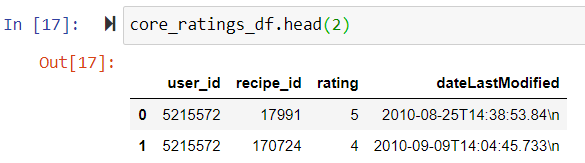
\includegraphics[width=0.8\linewidth]{raw_ratings_head}
	\caption{Raw User-Interaction Data}
	\label{fig:raw_ratings_head}
\end{figure}
\end{singlespace}

\subsection{Features Extraction}
A content-based filtering algorithm relies on the contents of the items. In our dataset, recipes are items that are rated by users. To recommend any recipe for a user, it is important to understand the features of the recipe that are relevant for a user. This thesis considers  `Ingredients', `Cook Method', `Calories' and `Diet Labels' features to find similarities between recipes.

\subsubsection{Ingredients Extraction}
The recipe's data received from Kaggle has the ingredients column in a clean format up to a certain level. To get a single ingredient for each recipe, the `NLTK' library has been used. It tokenizes sentences into words. Raw ingredients data has many irrelevant words for predicting similarity between ingredients such as `white' from `egg white', `frozen' from `frozen chicken', `thawed' from `thawed rotis', `piece from pork piece'. Such custom keywords are filtered out using a recipe\_stopwords list to make ingredients very specific. The difference between raw ingredients and cleaned ingredients is illustrated in \autoref{fig:raw_ingredients} \autoref{fig:clean_ingredients}. Irrelevant words such as `thawed' and `white' present in the first row of the pre-processed ingredients have been removed in post-processed ingredients. On this clean data, lemmatization is performed to transform a word into its existing word. Part-of-speech tags considered are `nouns' and `adjectives'. Example `potatoes' will be transformed to `potato' as show in \autoref{fig:lemma_ingredients}

\begin{singlespace}
\begin{figure}[H]
	\centering
	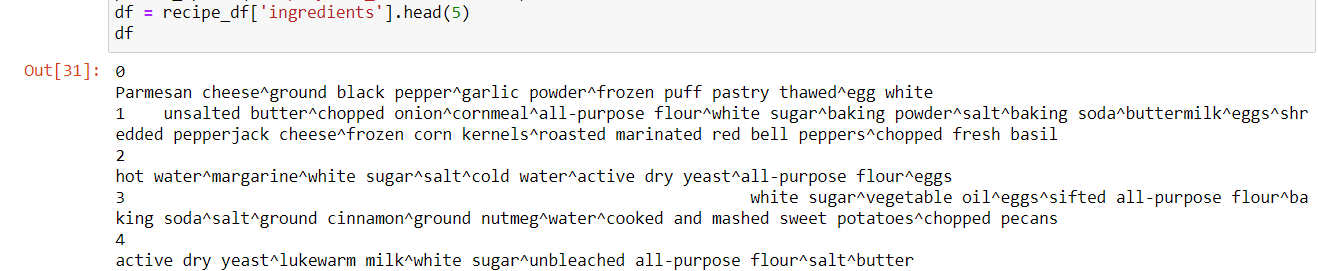
\includegraphics[width=1.0\linewidth]{raw_ingredients}
	\caption{Pre-Processed Ingredients }
	\label{fig:raw_ingredients}
\end{figure}  
\end{singlespace}
\begin{singlespace}
\begin{figure}[H]
	\centering
	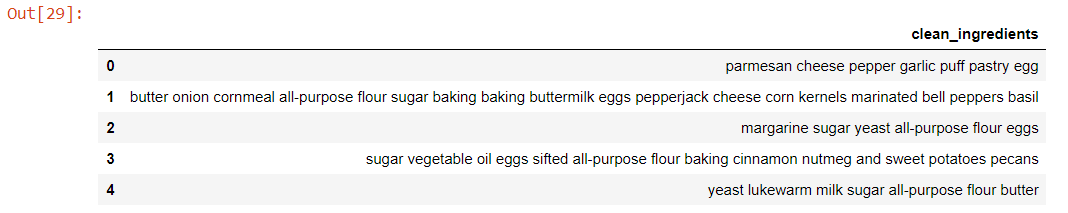
\includegraphics[width=1.0\linewidth]{clean_ingredients}
	\caption{Post-Processed Ingredients }
	\label{fig:clean_ingredients}
\end{figure}  
\end{singlespace}
\begin{singlespace}
\begin{figure}[H]
	\centering
	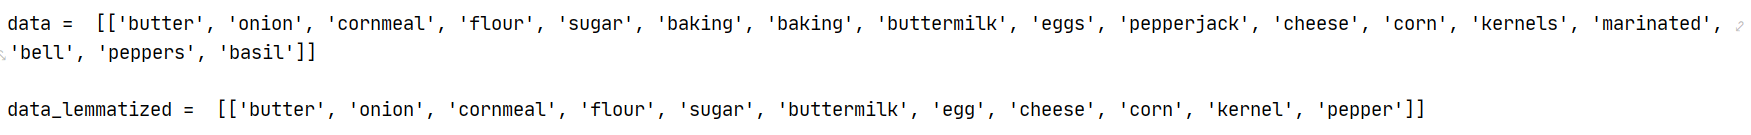
\includegraphics[width=1.0\linewidth]{lemma_ingredients}
	\caption{Post-Lemmatization Ingredients }
	\label{fig:lemma_ingredients}
\end{figure}  
\end{singlespace}

\subsubsection{Cook Method Extraction}
\label{sec:cook_method}
Ingredients are most significant in measuring the similarity between recipes but instead of only ingredients, Wang et al. [49] represented the recipes as graphs which are built on ingredients and cooking directions that can be used to easily aggregate dishes. 
The University of Minnesota has predefined glossary of cooking methods \cite{50} that has $74$ cooking methods such as `bake', `steam', `fry'. Recipes dataset of this thesis has a `cooking\_direction' column that contains the method of cooking. It is a set of sentences that provides all instructions for a recipe as shown in \autoref{fig:cooking_directions}.
\begin{singlespace}
\begin{figure}[H]
	\centering
	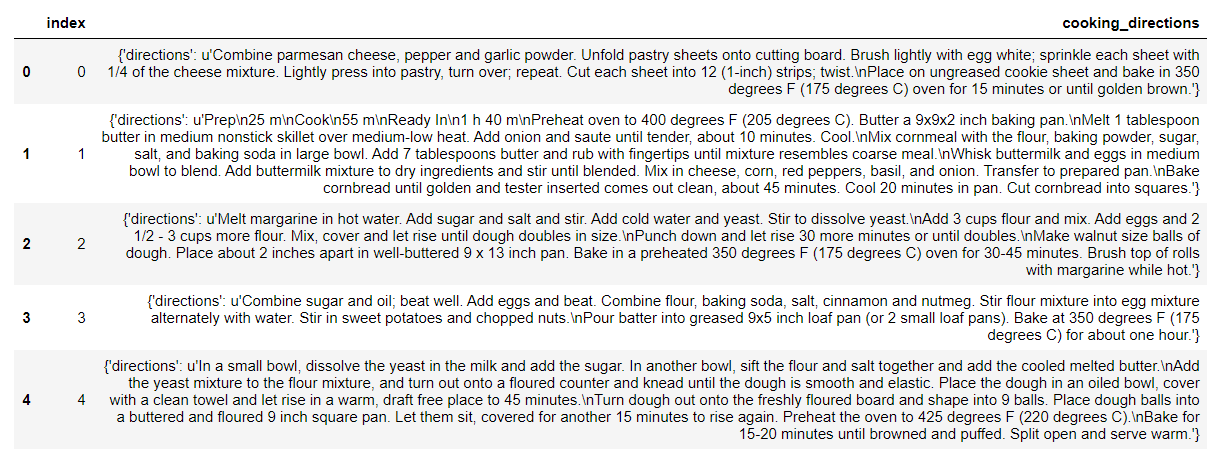
\includegraphics[width=1.0\linewidth]{cooking_directions}
	\caption{Cooking Directions }
	\label{fig:cooking_directions}
\end{figure}
\end{singlespace}

\noindent To get a cooking method from cooking direction, `NLTK Processing' is performed on `cooking\_direction' column.  The first step of this processing is to convert the set of instructions into words. Conversion of sentences to words is done using `NLTK Tokenizer.' The next step is to remove `stop words' from sentences. In natural language processing, stop words refer to words that do not have meaningful information such as `a', `and', `an', `the'. These words are considered as noisy data and can be ignored. These stopwords are downloaded from the `NLTK' library. The result is a list of keywords for cooking methods and ingredients. The common words from this result and predefined glossary of cooking methods are extracted and mapped as cooking methods used in the associated recipe. The list of cooking methods used in recipes is depicted in \autoref{fig:cooking_methods}.
\begin{singlespace}
\begin{figure}[H]
	\centering
	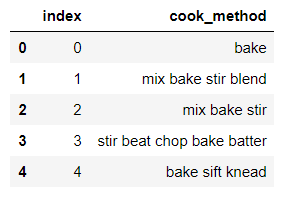
\includegraphics[width=0.5\linewidth]{cooking_methods}
	\caption{Cooking Methods }
	\label{fig:cooking_methods}
\end{figure}  
\end{singlespace}

\subsubsection{Calories Extraction}
A calorie is a unit of an energy. Calories in any food refers to the energy people get by consuming food. Recipe dataset has `nutrition' column. For each recipe, nutrition values are specified with quantity. For example, `Crispee Cheese twists' recipe has 121 calories as depicted in  \autoref{fig:nutritions}. This information is stored in a nested dictionary. After extracting calorie's information it is stored in the `calories' column as showin in \autoref{fig:calories}.
\begin{singlespace}
\begin{figure}[H]
	\centering
	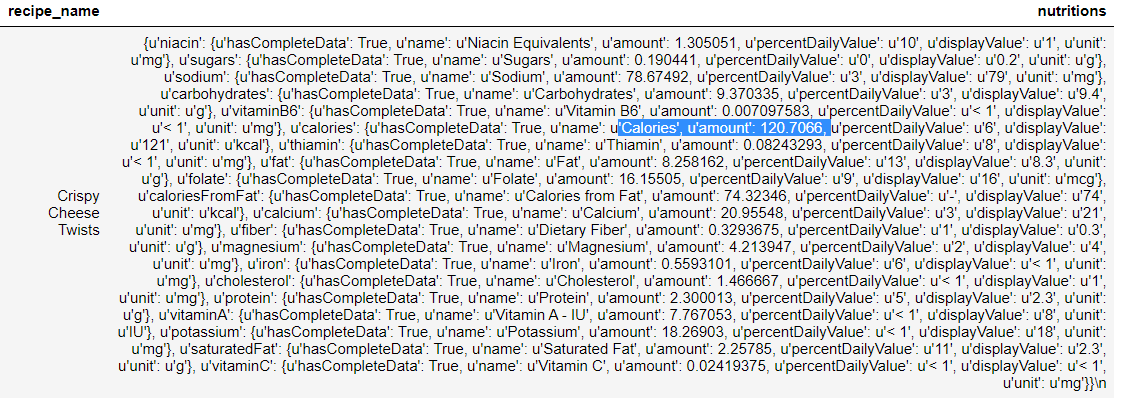
\includegraphics[width=1.0\linewidth]{nutritions}
	\caption{Recipe - Nutrition }
	\label{fig:nutritions}
\end{figure}  
\end{singlespace}
\begin{singlespace}
\begin{figure}[H]
	\centering
	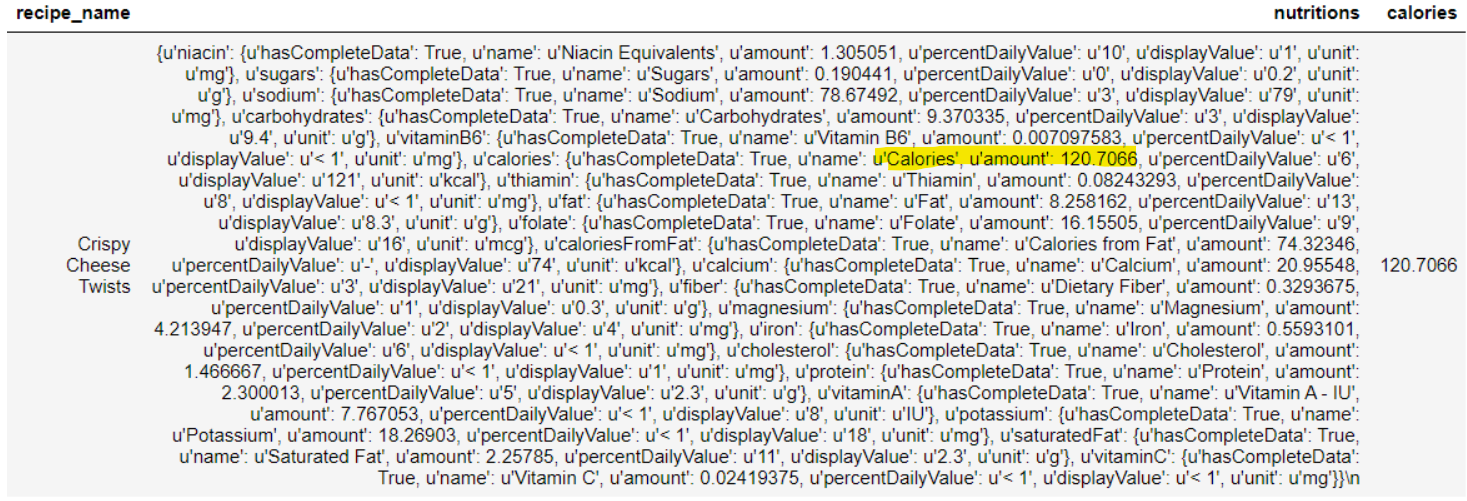
\includegraphics[width=1.0\linewidth]{calories}
	\caption{Recipe - Calories }
	\label{fig:calories}
\end{figure}  
\end{singlespace}

\subsubsection{Diet Labels Extraction}
\label{sec:diet_labels}
According to U.S. Food and Drug Administration (FDA) \cite{51}, \%DV is the percentage of the Daily Value for each nutrient in a serving of the food. Percentage Daily Value can inform if a serving of food is high or low in a nutrient. The general guide is, 5\% DV or less of a nutrient per serving is considered low and 20\% DV or more of a nutrient per serving is considered high. From this information, recipes are broadly divided into five categories such as \textbf{`highprotein'}, \textbf{`highfiber'}, \textbf{`lowfat'}, \textbf{`lowcarb'}, \textbf{`lowsodium'} and \textbf{`balanced'}. If \%DV value is less than 5\% then recipe will fall under low nutrition label category otherwise in high nutrition label category. For example, \autoref{fig:diet_labels} illustrates that for recipe `Crispee Cheese Twist', percentage daily value for carbohydrates is $3$ and for sodium is $3$ which is less than 5\%. Hence `Crispee Cheese Twist' will fall under `Low-Carb' and `Low-Sodium' category under column `diet\_labels'.
\begin{singlespace}
\begin{figure}[H]
	\centering
	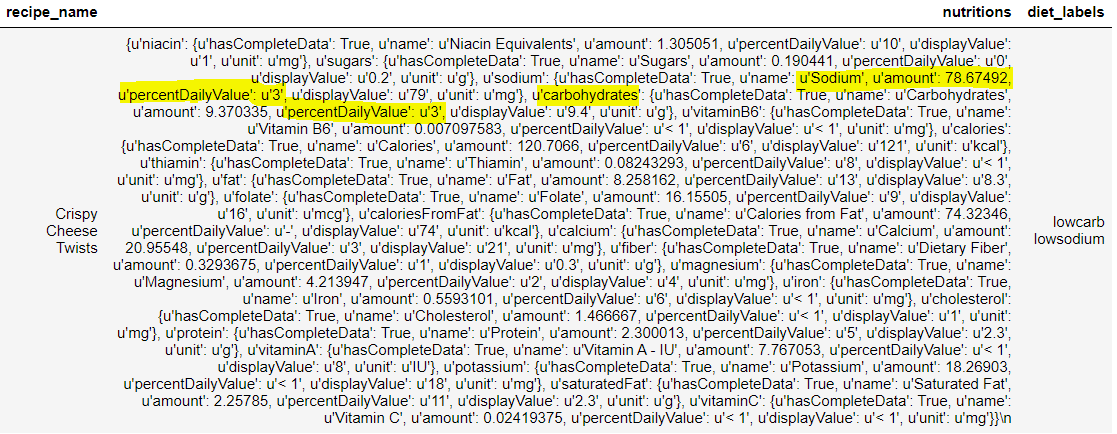
\includegraphics[width=1.0\linewidth]{diet_labels}
	\caption{Recipe - Diet Labels }
	\label{fig:diet_labels}
\end{figure}  
\end{singlespace}

\subsubsection{User Information}
\label{sec:user_info}
For a user `height\_in\_inches', `weight\_in\_lb', `age' in years, `gender' and `activity' attributes are considerd. An activity is divided into 5 categories. 1. Sedentary 2. Lightly Active 3. Moderately Active 4.Very Active 5. Extra Active. The user information such as height, weight, gender, age, activities is generated using python script. The height range for an adult is considered from 52 inches to 80 inches. The weight range for an adult is considered from 64 lbs to 175 lbs. The Harris–Benedict equation is used to estimate an individual's basal metabolic rate (BMR). This estimated BMR value multiplied by a number that corresponds to a user's activity level provides the approximate daily kilocalorie intake to maintain current body weight \cite{52}. To calculate BMR of male and female, the Harris–Benedict equation is given below.
\begin{align}
BMR (Male) = 66 + (6.3 * Weight\_lb) + (12.9 * Height\_inch) - (6.8 * age) \\
BMR (Female) = 655 + (4.3 * Weight\_lb) + (4.7 * Height\_inch) - (4.7 * age)
%\label{eq:bmr_female}
\end{align}
The relationship between BMR and user's activity level is depicted in \autoref{tb:calorie_intake}.  The approximate daily kilocalorie intake to maintain current body of a user, is product of BMR to lifestyle factor as shown in \autoref{tb:calorie_intake}. 
% Please add the following required packages to your document preamble:
% \usepackage[table,xcdraw]{xcolor}
% If you use beamer only pass "xcolor=table" option, i.e. \documentclass[xcolor=table]{beamer}
\begin{table}[H]
\centering
\begin{tabular}{|l|l|l|}
\hline
\rowcolor[HTML]{C0C0C0} 
{\color[HTML]{333333} \textbf{Lifestyle}} & {\color[HTML]{333333} \textbf{Multiplication Factor}} & {\color[HTML]{333333} \textbf{Approximate Calorie Intake}} \\ \hline
Sedentary                                 & 1.2                                                   & BMR * 1.2                                                  \\ \hline
Lightly Active                           & 1.375                                                 & BMR * 1.375                                                \\ \hline
Moderately Active                        & 1.55                                                  & BMR *1.55                                                  \\ \hline
Very Active                              & 1.725                                                 & BMR *1.725                                                 \\ \hline
Extra Active                         & 1.9                                                   & BMR *1.9                                                   \\ \hline
\end{tabular}
\caption{Calorie Intake based on BMR}
\label{tb:calorie_intake}
\end{table}
